% -----------------------------------------------
% Template for ISMIR Papers
% 2020 version, based on previous ISMIR templates

% Requirements :
% * 6+n page length maximum
% * 4MB maximum file size
% * Copyright note must appear in the bottom left corner of first page
% * Clearer statement about citing own work in anonymized submission
% (see conference website for additional details)
% -----------------------------------------------

\documentclass{article}
\usepackage[T1]{fontenc} % add special characters (e.g., umlaute)
\usepackage[utf8]{inputenc} % set utf-8 as default input encoding
\usepackage{ismir,amsmath,cite,url}
\usepackage{graphicx}
\usepackage{color}

% Optional: To use hyperref, uncomment the following.
% \usepackage[bookmarks=false,hidelinks]{hyperref}
% Mind the bookmarks=false option; bookmarks are incompatible with ismir.sty.

\usepackage{lineno}
\linenumbers

% Title.
% ------
\title{Neural models for computer-assisted musical orchestration: a preliminary study}

% Note: Please do NOT use \thanks or a \footnote in any of the author markup

% Single address
% To use with only one author or several with the same address
% ---------------
%\oneauthor
% {Names should be omitted for double-blind reviewing}
% {Affiliations should be omitted for double-blind reviewing}

% Two addresses
% --------------
%\twoauthors
%  {First author} {School \\ Department}
%  {Second author} {Company \\ Address}

%% To make customize author list in Creative Common license, uncomment and customize the next line
%  \def\authorname{First Author, Second Author}


% Three addresses
% --------------
\threeauthors
  {First Author} {Affiliation1 \\ {\tt author1@ismir.edu}}
  {Second Author} {\bf Retain these fake authors in\\\bf submission to preserve the formatting}
  {Third Author} {Affiliation3 \\ {\tt author3@ismir.edu}}

%% To make customize author list in Creative Common license, uncomment and customize the next line
%  \def\authorname{First Author, Second Author, Third Author}

% Four or more addresses
% OR alternative format for large number of co-authors
% ------------
%\multauthor
%{First author$^1$ \hspace{1cm} Second author$^1$ \hspace{1cm} Third author$^2$} { \bfseries{Fourth author$^3$ \hspace{1cm} Fifth author$^2$ \hspace{1cm} Sixth author$^1$}\\
%  $^1$ Department of Computer Science, University , Country\\
%$^2$ International Laboratories, City, Country\\
%$^3$  Company, Address\\
%{\tt\small CorrespondenceAuthor@ismir.edu, PossibleOtherAuthor@ismir.edu}
%}
%\def\authorname{First author, Second author, Third author, Fourth author, Fifth author, Sixth author}


\sloppy % please retain sloppy command for improved formatting

\begin{document}

%
\maketitle
%
\begin{abstract}
In this paper we will explore preliminary neural models for the task of computer-assisted musical orchestration. After an introduction on the problem, we will show how we decided to model musical orchestration as a classification task. In this context, we will propose two deep learning models and we will show how they perform as classifiers for musical instruments recognition by comparing them with specific baselines. We will the show how they perform, both qualitative and quantitative, in the task of computer-assisted orchestration by comparing them with state-of-the-art systems. We will highlight, finally, benefits and problems of neural approaches for orchestration and we will propose possible future steps.

\end{abstract}
%
\section{Introduction}\label{sec:introduction}

\section{Data generation}
We used the TinySOL database to create our input data. TinySOL is a subset of the Studio On Line (SOL) database created by IRCAM. TinySOL contains 2,478 samples from 12 instruments. The instruments come from different orchestral families: strings, woodwinds, and brass are all represented in TinySOL. Each TinySOL sample is one instrument playing one note in the "ordinary" playing style.

When training a model, the number of samples $n$ to be used in each combination is specified. To create the training data, $n$ instruments are randomly selected from the list of specified instruments, and then a TinySOL sample is randomly selected for each chosen instrument. This gives $n$ different samples, each of a different instrument. These samples are combined to form a soundfile that has each sample playing simultaneously. The audio was trimmed to four seconds in length so our data would all be of the same size. The melspectrogram is taken of this combination, creating the features to be fed to the model. We created the melspectrogram by \textbf{(Alejandro can you write this of how you generated the melspectrograms using the STFT?)}. We chose to use the melspectrogram because of its ability to represent timbre, a key part of assisted orchestration.

\section{Our model}
- deep learning trained for classification and then used for orchestraion
- changing number of instruments

Our idea is to perform orchestration using deep neural networks trained for classification. By generating input data that is a mixture of different instruments and pitches, the network learns how to take a sound that is a complex combination of notes and timbres and deconstruct it into its original parts. When a target sound is then fed to the network, it attempts to classify which samples would best represent the target. By taking the samples that have the highest probability of being in the target, an orchestrated solution can be created. 

We did not train our model to classify the dynamics of a sample despite TinySOL having pianissimo, mezzo forte, and fortissimo recordings for each sample. If we had, then each class would have only one data point. Instead, when the model is used for orchestration, the dynamic is determined by the probability of that sample as output by the model. If the model output a probability higher than $0.66$ for a sample, the fortissimo version of the sample was used. If it was between $0.33$ and $0.66$, then the mezzo forte version, and if less than $0.33$ the pianissimo dynamic.

\subsection{Baseline}
In order to have a baseline to compare our results against, we attempted to solve the classification problem using various parametric classifiers. The classifiers we tested were Support Vector Machine (SVM), Random Forest, and K-Nearest Neighbors. We used the implementations provided in the scikit-learn library for each classifier. For SVM, we used SVC with an RBF kernel. For Random Forest, we set the maximum depth of each tree to be 15. Each classifier was wrapped in a MultiOutputClassifier to achieve the multi-label nature of this problem. We found SVM to have the highest accuracy of the three classifiers across all experiments. All of the following baseline experiments used 50,000 generated samples with a train-test split of 60/40. Each sample is a combination of one or more instruments and is four seconds in length. The features used are the mel frequency cepstral coefficients (MFCCs) of the resulting combination, with a total of 100 coefficients per sample. We chose MFCCs because of their ability to describe the timbre of a sample using a relatively small number of coefficients.

We started by simplifying the problem to classifying only the instruments and not the pitch. This had the benefit of both reducing the number of classes and increasing the number of samples per class. We found that SVM was able to very accurately identify the instrument given an input that had only one instrument present; for this case the accuracy was 99.8\%. However as soon as multiple instruments were present in the input, the accuracy dropped significantly. With two instruments, accuracy was 55.4\%, with three it was 19.6\% and with 10 instruments the accuracy was 0.5\%. 

To better approximate the problem of identifying instrument and pitch, we then attempted to classify the instrument and pitch class. That is, which octave the pitch was in did not matter, only the pitch class. The input was a combination of two instruments drawn from a possible twelve instruments, and the classifier attempted to identify which instruments were present and for two of those instruments, say Flute and Violin, which pitch classes were present. If another instrument was present that was not Flute or Violin, the classifier would attempt to identify that instrument, but not its pitch class. The best results from this setting of the problem was SVM with 30.2\% accuracy, which was a result of classifying the pitch class of Flute and Violin. Depending on which two instruments had their pitch class identified, the accuracy varied greatly. For a Violin and Cello accuracy was 20.9\%, and for Trombone and Bass Tuba accuracy was 2.2\%.

For a slight modification on this setting, we no longer attempted to identify which instrument was present if it was not one of the two instruments whose pitch class was being identified. Instead, the classifier would simply identify that an instrument that was not one of the two was present. Since this is a simpler problem, it lead to increased accuracies. The accuracies from this experiment are outlined in Table 1.

We then performed this same experiment with three instruments having their pitch class identified. Each input was a combination of three instruments drawn from a possible twelve instruments. For three instruments specified in that experiment, pitch class was identified. Flute, Oboe, and Violin reached an accuracy of 11.1\%, and Bass Tuba, Trumpet, and Trombone was 0.5\%. As we increased the number of instruments whose pitch classes was being identified, the accuracy continued to drop. For classifying the pitch class of four instruments: Oboe, French Horn, Violin, and Flute, the accuracy was 2.7\%.

This was still a simplified version of the problem, as we were identifying only the pitch class of a few instruments. However, the parametric classifiers were unable to achieve accurate results as the number of instruments increased. Therefore, we did not attempt the full setting of the problem, in which individual pitches are classified for all instruments, with parametric classifiers. 

\begin{table}
  \begin{center}
    \label{tab:table1}
    \begin{tabular}{|c|c|c|c|} 
    	  \hline
      \textbf{Instr. 1} & \textbf{Instr. 2} & \textbf{SVM Accuracy} & \textbf{RF Accuracy}\\
      \hline
      Violin & Flute & 38.8\% & 9.8\% \\
      \hline
      Violin & Trumpet & 33.8\% & 9.1\% \\
      \hline
      Violin & Cello & 34.8\% & 6.3\% \\
      \hline
      Cello & Viola & 32.1\% & 5.8\% \\
      \hline
      Oboe & French Horn & \textbf{39.9\%} & \textbf{17.5\%} \\
      \hline
    \end{tabular}
  \end{center}
  \caption{Comparison of results between SVM and Random Forest. Each data point is a combination of two TinySOL samples, where at least one of the samples is from one of the two instruments specified for that experiment. For the samples drawn from one of the two instruments, the pitch class of that sample is identified. For a sample not from one of the two instruments, the classifier simply attempted to identify that a sample from one of the non-specified instruments was present. In this setting, there are 25 classes: 24 from the 12 pitch classes from 2 instruments, and 1 class that specified whether an instrument that is not one of the two specified is present.}
\end{table}



\subsection{CNN with LSTM}

The first deep model we examined was a Convolutional Neural Network (CNN). CNN shows good performance on classification assignment for its strong ability to extract local features, so we implemented a basic CNN with three convolutional layers and two fully connected layers. Each convolutional layer is followed by a BatchNorm layer, a ReLU activation layer and a $2 \times 2$  MaxPool layer with a stride of 2. The kernel size is $3 \times 3$ with a stride of 1 and a padding of 1. The number of filters are 8, 16, 32. This setting is simple but we can make a good comparison between it and the baseline. 

\begin{figure*}[ht]
\centering
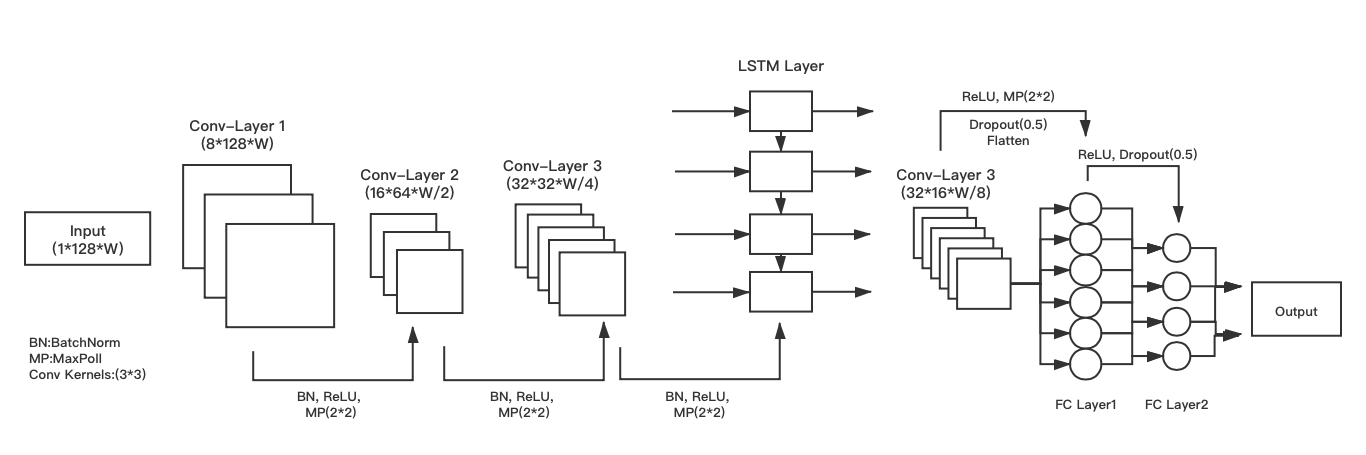
\includegraphics[scale=0.35]{figs/CNN_with_LSTM.png}
\caption{Model Architecture}
\label{cnn_lstm}
\end{figure*}

Given that audio is one kind of sequential data, it is easy to consider Long Short-Term Memory network (LSTM) as a choice of modeling sequential data. In our setting, we added one LSTM layer with 32 outputs units following three convolutional layers. The convolutional layers did not change the sequence relationship. Instead, it scaled down the size of feature maps. After LSTM layer, we reshaped the output into the same size before inputing. Then we implemented another convolutional layer with the same structure and kernel size. Finally, we flattened out the outputs and fed them into fully connected layers with Dropout layer. The probability of an element to be zeroed is 0.5 and we took sigmoid as activation function. Since there is no competition relationship between different classes for each class can be classification result equally, it is reasonable for us to take sigmoid activations and used binary classification for each class to treat them independently. We minimize the binary cross entropy(BCE) loss between the predictions and targets. We implemented our neural networks with PyTorch and trained them with Adam optimizer. The model architecture is shown in Figure\ref{cnn_lstm}.  



\subsection{ResNet}
- SVM was good but CNN was better and ResNet was best
- review all experiments we did and choose key plots

To make our setting more reasonable, we took the well-known deep residual network(ResNet) as backbone in our experiments. Specifically, we used 18-layer ResNet, which allows information to pass directly from the input to the final layer of each block. Besides, to make the model more suitable to our problem, we reduce the number of parameters and reset the output channel numbers of each block with 32, 64, 32, 32 respectively. We took the same loss function-BCE and optimizer-Adam as those in training the CNN with LSTM model.

\section{Orchestration experiments}
- set of 10 targets
- orchestra fix to 10
- qualitative evaluation: acoustic inspection of the solutions
- quantitative evaluation: distance in feature space
- comparison table between Orchidea and our model

Our final model was trained on data where each input was a combination of ten instruments, but we performed experiments with varying numbers of instruments used in combination. (insert table of data showing the results of CNN with 2,3,4 etc instruments) An arbitrary number of samples can be used in the solution, since the $n$ highest probabilities can be taken from the output, leading to $n$ samples in the solution.

We tested our models using 15 targets for orchestration. Two of the targets were made from TinySOL samples, but the rest are not combinations of input data, and some are not even recordings of instruments. Among the targets are recordings of bells, a car horn, a gong, and a recording of a boat docking. By passing these samples into a model, an orchestration of the target is created from the TinySOL samples that were used to train the network. 

For orchestrating these targets, we used both the CNN and ResNet models. The CNN was trained on 200,000 samples for 49 epochs and the ResNet on 400,000 samples for 24 epochs. The instruments used to train the models are: French Horn, Oboe, Violin, Viola, Cello, Flute, Trombone, Bassoon, Trumpet, and Clarinet. The resulting orchestrations are made from 10 samples drawn from these instruments.

Although the data we trained the model on was fixed to four seconds of audio, the target samples can be of arbitrary length. By changing the mel hop length, which is the distance between the frames of the melspectrogram, an audio signal of any length can be represented as a matrix of the same size as the training data.

\subsection{Evaluation}
-evaluation of orchestrations (not evaluation of model)

We evaluated our orchestrations both qualitatively and quantitatively. Qualitative evaluation was done through an acoustic inspection of the solution, paying close attention to both timbre and pitch. For targets that had harmonic content, it was noted if the partials present in the target were also represented in the orchestrated solution.

For quantitative evaluation, we used the distance metric defined in \eqref{distance} to calculate the distance between the target samples and our orchestrated solutions. We then orchestrated the same targets with OrchIdea and calculated the distance for OrchIdea's solutions. A comparison of these results is in Table 2.

\begin{equation}\label{distance}
d(x, \tilde{x}) =\lambda_1 \sum_k \delta_{k1}(x_k - \tilde{x}_k) + \lambda_2 \sum_k \delta_{k2}|x_k - \tilde{x	}_k| \\
\end{equation}

$$
\delta_{k1} = 
\begin{cases}
1, \text{if   } x_k > \tilde{x}_k \\
0, \text{otherwise}
\end{cases} 
$$

$$
\delta_{k2} = 
\begin{cases}
1, \text{if   } x_k < \tilde{x}_k \\
0, \text{otherwise}
\end{cases} 
$$


This metric computes the difference between the FFT of the target and the FFT of the solution. 

\textbf{(Add results of quantitatively comparing our results to OrchIdea)}

\begin{table}
  \begin{center}
    \label{tab:table2}
    \begin{tabular}{|c|c|} 
    	  \hline
      \textbf{Model} & \textbf{Average Distance} \\
      \hline
      CNN with LSTM &   \\
      \hline
      ResNet &  \\
      \hline
      OrchIdea &  \\
      \hline
    \end{tabular}
  \end{center}
  \caption{Comparison of the orchestration solutions of our two models, CNN with LSTM and ResNet, against OrchIdea's solutions. The distance between the target and solution are calculated for each target using \eqref{distance} and then averaged.}
\end{table}



\section{Evaluation and Conclusions}
- the approach seems promising for orchestration
- many things used in Orchidea are not implemented here (symbolic constraints, sparsity,...)
- CNN seems better for timbre
- ResNet seems better for pitch (what are timbre and pitch??)

Based on our accuracies from training the model and the results of orchestrating 15 targets, our approach seems promising for orchestration. When comparing our method with OrchIdea, it is important to note that many of the processes OrchIdea uses to optimize its solution were not used in our model. This includes important aspects such as sparsity, partial filtering, \textbf{(Carmine any more to add?)}. Our model also lacks the implementation of symbolic constraints, which is an important part of assisted orchestration.

In order to have comparable solutions, we did not allow OrchIdea to create sparse solutions, meaning that OrchIdea was forced to use all 10 instruments in each solution. This creates a more fair comparison since our model is optimize solutions by using fewer than 10 samples.

\textbf{(Alejandro, add how there were certain instruments that performed really poorly or really well. Add how ResNet was awful for Flute and always output Flute C7)}

We find that the CNN and ResNet give similar accuracies during training, but perform differently when tasked with orchestrating targets. Overall, CNN seems to better emulate the timbre in its orchestrations, where ResNet is better for recreating the pitch of the target. For a target that contained specific notes, the solution from ResNet contained both the note in the target and its partials: a sample that was two octaves higher, the fifth an octave up, and a minor third two octaves up (mix\_ObA4\_BnC3). Clearly, ResNet was able to identify the partials of the target and recreate them in the solution.

\subsection{Interpreting the Latent Space}
- the system finds filters like...

\section{Future steps}
- using conditioning to impose symbolic constraints
- variable size solutions
- joint networks for orchestral size detection and orchestral families (see paper)

Future steps in this project include implementing various methods that are present in OrchIdea. 

Our current model orchestrates all targets using the same number of samples, and this does not take into account the density of different targets. The solution to this is to allow sparse solutions in which the model decides how many samples should be used to best represent the target. This allows a small number of samples to be used for sonically sparse sounds and many to be used for sonically dense sounds. 

Partial filtering is a method that would aid our model in orchestrating the harmonics of a target. The dominant harmonic partials of the target are identified, and the search space is limited to only include samples of those pitches. For example, if the target is a recording of an instrument playing a C4, then the partials identified may be C4, C5, G5, and E6. The model would then only consider samples of these pitches to be used in the solution. This leads to a solution whose harmonics are much closer to the target, which is an important part of aural similarity.

\section{Citations}

All bibliographical references should be listed at the end,
inside a section named ``REFERENCES,'' numbered and in alphabetical order.
All references listed should be cited in the text.
When referring to a document, type the number in square brackets
\cite{Author:00}, or for a range \cite{Author:00,Someone:10,Someone:04}.

When the following words appear in the conference publication titles, please abbreviate them: Proceedings $\rightarrow$ Proc.; Record $\rightarrow$ Rec.; Symposium $\rightarrow$ Symp.; Technical Digest $\rightarrow$ Tech. Dig.; Technical Paper $\rightarrow$ Tech. Paper; First $\rightarrow$ 1st; Second $\rightarrow$ 2nd; Third $\rightarrow$ 3rd; Fourth/nth $\rightarrow$ 4th/nth.

\textcolor{red}{As submission is double blind, refer to your own published work in the third person. That is, use ``In the previous work of \cite{Someone:10},'' not ``In our previous work \cite{Someone:10}.'' If you cite your other papers that are not widely available (e.g., a journal paper under review), use anonymous author names in the citation, e.g., an author of the form ``A. Anonymous.''}

% For bibtex users:
\bibliography{ISMIRtemplate}

% For non bibtex users:
%\begin{thebibliography}{citations}
%
%\bibitem {Author:00}
%E. Author.
%``The Title of the Conference Paper,''
%{\it Proceedings of the International Symposium
%on Music Information Retrieval}, pp.~000--111, 2000.
%
%\bibitem{Someone:10}
%A. Someone, B. Someone, and C. Someone.
%``The Title of the Journal Paper,''
%{\it Journal of New Music Research},
%Vol.~A, No.~B, pp.~111--222, 2010.
%
%\bibitem{Someone:04} X. Someone and Y. Someone. {\it Title of the Book},
%    Editorial Acme, Porto, 2012.
%
%\end{thebibliography}

\end{document}

